\section{Post-Double Lasso (Double Selection) with High-Dimensional Controls}


\begin{quotation}
\noindent The abundance of data and resources facilitates the move away from a deductive social science to a more sequetial, interactive, and ultimately inductive approach to inference.
\\ \cite{grimmer2021machine}
\end{quotation}


\begin{quotation}
\noindent We hope readers will that data mining done correctly is the opposite of ``bad practice.'' \\  \cite{belloni2014high} 
\end{quotation}

\subsection*{Practical guide}

Partially linear model with many controls
\[
y_i=\alpha_0 d_i + x_i'\beta_0 + \zeta_i,\qquad
d_i=x_i'\pi_0+v_i,\qquad \mathbb{E}[\zeta_i\mid d_i,x_i]=\mathbb{E}[v_i\mid x_i]=0.
\]

In a typical application, we are interested in the effect, $\alpha_0$ of a treatment variable $d$. The vector of covariates $x$ is included to control for confounding. 
In your data, there might be more predictors than $n$ observations. However, proceeding with double lasso involves a structural assumption that $y$ and $d$ depend only on a subset of predictors that is necessarily less than $n$.

\paragraph{Algorithm (post-double lasso).}
\begin{enumerate}
\item \textbf{Outcome lasso:} Regress $y$ on $x$ via lasso (or square-root lasso). Let $\widehat S_y=\{j:\widehat\beta_{y,j}\neq 0\}$.
\item \textbf{Treatment lasso:} Regress $d$ on $x$ via lasso. Let $\widehat S_d=\{j:\widehat\pi_{d,j}\neq 0\}$.
\item \textbf{Union:} $\widehat S=\widehat S_y\cup \widehat S_d$ \emph{(optionally augment by a small ``amelioration'' set you insist on keeping).}
\item \textbf{Final OLS (unpenalized):} Regress $y$ on $\{d, x_{\widehat S}\}$. The coefficient on $d$ is $\widehat\alpha$.
\end{enumerate}

\paragraph{Multiple target regressors (e.g., interactions).}
If the final specification includes a small, fixed set of target regressors (e.g., $d$ and an interaction $d\times e$), run step 2 separately for \emph{each}, 
union all selected controls with $\widehat S_y$, and run the final OLS of $y$ on $W$ and $x_{\widehat S}$.

\paragraph{Penalty level and loadings (lasso tuning).}
Use predictor-specific \emph{penalty loadings}, which vary the regularization penalty for each variable. Solve
\[
\min_b\  \|y-Xb\|_2^2 + \lambda \sum_{j=1}^p \hat\ell_j\,|b_j|,
\]

\cite{belloni2014inference} uses
\[
\lambda = 2c\,\sqrt{n}\,\Phi^{-1}\!\Big(1-\frac{\gamma}{2p}\Big),\qquad
\hat\ell_j = \sqrt{\mathbb{E}_n[x_{ij}^2\,\hat\varepsilon_i^2]}\ ,
\]
where $\hat\varepsilon$ are residuals from a post-lasso fit.

\subsection*{Assumptions}

%\paragraph{Baseline (as in textbook OLS for the partially linear estimand).}
%\begin{enumerate}
%\item \textbf{Exogeneity:} $\mathbb{E}[\zeta_i\mid d_i,x_i]=0$ (controls are pre-treatment).
%\item \textbf{Overlap/variation:} $\mathbb{E}[(d_i-\mathbb{E}[d_i\mid x_i])^2]\ge c>0$ (residual variance of $d$ given $x$ is not vanishing).
%\item \textbf{Moments:} Finite second (often a bit higher) moments; heteroskedasticity allowed (use robust SE).
%\end{enumerate}

%\paragraph{Additional for post-double lasso.}
Typical OLS assumptions \emph{and} \cite{belloni2014inference} lists several technical conditions that are sufficient for valid inference. 

\begin{enumerate}
\item \textbf{Approximate sparsity:} There exist sparse $\beta_0,\pi_0$; approximation errors don't grow ``too fast.''
\item \textbf{Restricted eigenvalue/compatibility:} Design of $X$ is ``nice'' (well-conditioned sparse Gram submatrices).
\item \textbf{Rates:} The strongest condition is $s^2\log^2(p\vee n)/n\to 0$, where $s$ is the number of selected controls and $p$ is the total considered. These can't be too big relative to $n$.
\item \textbf{Penalty calibration:} $\lambda$ of the same order as $\sqrt{n\log p}$ and heteroskedastic-robust loadings $\hat\ell_j$ (feasible, iterated) to control the coordinate-wise score.
\end{enumerate}

\bigskip

\subsection*{Technical intuition}

\paragraph{Orthogonal (Neyman) score.} Define
\[
\psi_i(\alpha,\beta,\pi)=(y_i-\alpha d_i - x_i'\beta)\,(d_i-x_i'\pi).
\]
At the true parameter values $(\alpha_0,\beta_0,\pi_0)$ one has $\mathbb{E}[\psi_i]=0$ \emph{and} this makes the estimating equation \emph{insensitive} (to first order) to small errors in the high-dimensional nuisances $(\beta,\pi)$.
Double selection implements this orthogonality. Under our assumptions, and the excluded controls should have very small effects and errors are second order. 

\paragraph{Bias decomposition via FWL.} Let $S=\widehat S_y\cup \widehat S_d$ and $M_S=I-X_S(X_S'X_S)^{-1}X_S'$ be the residual-maker for $X_S$. Then the final OLS coefficient obeys
\[
\widehat\alpha-\alpha_0
=\underbrace{\frac{d'M_S X\beta_0}{d'M_S d}}_{\text{bias from omitted $X\beta_0$ after selection}}
+\underbrace{\frac{d'M_S \zeta}{d'M_S d}}_{\text{mean-zero noise (drives SE)}}.
\]

This can be bound and the asympotitic properties understood.

\section{Logistic Regression}

Logistic regression is used to predict a binary target variable. 

%$$y_i = \frac{1}{1 + e^{-w^T x_i}}$$
$$p_i=\Pr(y_i=1\mid x_i)=\frac{1}{1+e^{-w^\top x_i}}.$$


With $x_i \in \mathbb{R}^d$, we have parameters $w \in \mathbb{R}^d$. 

The right hand side is the logistic function. Its inverse is the logit function, $\text{logit}(p) = \log \frac{p}{1-p}$.

Recall this logistic form implies the log odds are linear in $x$:
$$\text{logit}(p) = w^T x.$$


\subsection{Example}

Though it's a bit silly to run a logistic regression with an intercept and a single binary independent variable, it provides a useful toy example. 

Suppose we have the following data:

\begin{center}
\begin{tabular}{ccc}
\toprule 
No.\ Observations & $x$ & $y$ \\
\midrule
9 & 0 & 0 \\
1 & 0 & 1 \\
1 & 1 & 0 \\
9 & 1 & 1 \\
\bottomrule
\end{tabular}
\end{center}

We observe $y=1$ 10\% of the time if $x=0$ and $y=1$ 90\% of the time if $x=1$. The log odds are $-2.2$ and $2.2$, respectively. With just two points in $x$ and log odds space, we can find the line by hand. The intercept is $-2.2$ and the slope is $4.4$. For an observation where $x_i=0$, then 
$(-2.2, 4.4) \begin{pmatrix} 1 \\ 0 \end{pmatrix} = (-2.2)(1) + (4.4)(0) = -2.2.$ The predicted probability is 0.1. 

Using a cutoff of $0.5$, we can create a confusion matrix and calculate some typical performance metrics for the training data. 

\begin{center}
\begin{tabular}{cc|cc}
& & \multicolumn{2}{c}{Predicted} \\
& & 0 & 1 \\
\midrule
\multirow{2}{*}{Actual} & 0 & 9 & 1 \\
& 1 & 1 & 9 \\
\end{tabular}
\end{center}

From this confusion matrix:
\begin{itemize}
\item Accuracy = $\frac{9 + 9}{20} = 0.90$
\item Precision = $\frac{9}{9 + 1} = 0.90$ 
\item Recall = $\frac{9}{9 + 1} = 0.90$
\item F1 = $\frac{2 \times 0.90 \times 0.90}{0.90 + 0.90} = 0.90$
\end{itemize}

The ROC AUC is $0.9$.

\begin{center}% requires \usepackage{pgfplots}
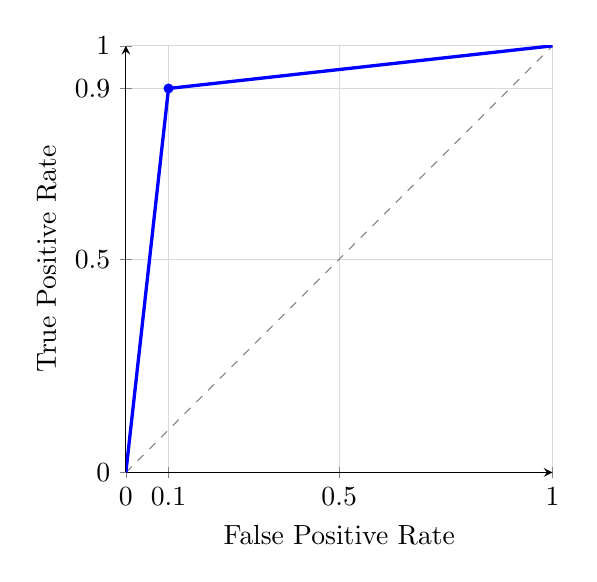
\begin{tikzpicture}
\begin{axis}[
  width=7cm,height=7cm, xmin=0,xmax=1, ymin=0,ymax=1,
  xlabel={False Positive Rate}, ylabel={True Positive Rate},
  grid=both, grid style={draw=gray!30}, axis lines=left,
  xtick={0,0.1,0.5,1}, ytick={0,0.5,0.9,1}
]
\addplot[dashed,gray] coordinates {(0,0) (1,1)};
% step path
\addplot[very thick,blue] coordinates {(0,0) (0.1,0.9) (1,1)};
% mark the 0.5 cutoff
\addplot[only marks, mark=*, mark size=1.6pt, blue] coordinates {(0.1,0.9)};
%\node[anchor=west] at (axis cs:0.12,0.88) {$t=0.5$ (FP=1, FN=1)};
%\node[anchor=west, blue] at (axis cs:0.04,0.75) {AUC = 0.90};
\end{axis}
\end{tikzpicture}
\end{center}

\subsubsection{Imbalance}

The previous example was one of \emph{class balance}. Now we add more cases of a negative label, on net, by increasing the number of observations where $x=0$ by a factor of $k$.

\begin{center}
\begin{tabular}{ccc}
\toprule 
No.\ Observations & $x$ & $y$ \\
\midrule
$9k$ & 0 & 0 \\
$1k$ & 0 & 1 \\
1 & 1 & 0 \\
9 & 1 & 1 \\
\bottomrule
\end{tabular}
\end{center}


Does that change the fitted line? Not at all, because we still have the same two points in $x$ and log odds space. However, performance metrics degrade. 




